%% This file was auto-generated by IPython.
%% Conversion from the original notebook file:
%% parallel.ipynb
%%
\documentclass[11pt,english]{article}

%% This is the automatic preamble used by IPython.  Note that it does *not*
%% include a documentclass declaration, that is added at runtime to the overall
%% document.

\usepackage{amsmath}
\usepackage{amssymb}
\usepackage{graphicx}
\usepackage{ucs}
\usepackage[utf8x]{inputenc}

% needed for markdown enumerations to work
\usepackage{enumerate}

% Slightly bigger margins than the latex defaults
\usepackage{geometry}
\geometry{verbose,tmargin=3cm,bmargin=3cm,lmargin=2.5cm,rmargin=2.5cm}

% Define a few colors for use in code, links and cell shading
\usepackage{color}
\definecolor{orange}{cmyk}{0,0.4,0.8,0.2}
\definecolor{darkorange}{rgb}{.71,0.21,0.01}
\definecolor{darkgreen}{rgb}{.12,.54,.11}
\definecolor{myteal}{rgb}{.26, .44, .56}
\definecolor{gray}{gray}{0.45}
\definecolor{lightgray}{gray}{.95}
\definecolor{mediumgray}{gray}{.8}
\definecolor{inputbackground}{rgb}{.95, .95, .85}
\definecolor{outputbackground}{rgb}{.95, .95, .95}
\definecolor{traceback}{rgb}{1, .95, .95}

% Framed environments for code cells (inputs, outputs, errors, ...).  The
% various uses of \unskip (or not) at the end were fine-tuned by hand, so don't
% randomly change them unless you're sure of the effect it will have.
\usepackage{framed}

% remove extraneous vertical space in boxes
\setlength\fboxsep{0pt}

% codecell is the whole input+output set of blocks that a Code cell can
% generate.

% TODO: unfortunately, it seems that using a framed codecell environment breaks
% the ability of the frames inside of it to be broken across pages.  This
% causes at least the problem of having lots of empty space at the bottom of
% pages as new frames are moved to the next page, and if a single frame is too
% long to fit on a page, will completely stop latex from compiling the
% document.  So unless we figure out a solution to this, we'll have to instead
% leave the codecell env. as empty.  I'm keeping the original codecell
% definition here (a thin vertical bar) for reference, in case we find a
% solution to the page break issue.

%% \newenvironment{codecell}{%
%%     \def\FrameCommand{\color{mediumgray} \vrule width 1pt \hspace{5pt}}%
%%    \MakeFramed{\vspace{-0.5em}}}
%%  {\unskip\endMakeFramed}

% For now, make this a no-op...
\newenvironment{codecell}{}

 \newenvironment{codeinput}{%
   \def\FrameCommand{\colorbox{inputbackground}}%
   \MakeFramed{\advance\hsize-\width \FrameRestore}}
 {\unskip\endMakeFramed}

\newenvironment{codeoutput}{%
   \def\FrameCommand{\colorbox{outputbackground}}%
   \vspace{-1.4em}
   \MakeFramed{\advance\hsize-\width \FrameRestore}}
 {\unskip\medskip\endMakeFramed}

\newenvironment{traceback}{%
   \def\FrameCommand{\colorbox{traceback}}%
   \MakeFramed{\advance\hsize-\width \FrameRestore}}
 {\endMakeFramed}

% Use and configure listings package for nicely formatted code
\usepackage{listingsutf8}
\lstset{
  language=python,
  inputencoding=utf8x,
  extendedchars=\true,
  aboveskip=\smallskipamount,
  belowskip=\smallskipamount,
  xleftmargin=2mm,
  breaklines=true,
  basicstyle=\small \ttfamily,
  showstringspaces=false,
  keywordstyle=\color{blue}\bfseries,
  commentstyle=\color{myteal},
  stringstyle=\color{darkgreen},
  identifierstyle=\color{darkorange},
  columns=fullflexible,  % tighter character kerning, like verb
}

% The hyperref package gives us a pdf with properly built
% internal navigation ('pdf bookmarks' for the table of contents,
% internal cross-reference links, web links for URLs, etc.)
\usepackage{hyperref}
\hypersetup{
  breaklinks=true,  % so long urls are correctly broken across lines
  colorlinks=true,
  urlcolor=blue,
  linkcolor=darkorange,
  citecolor=darkgreen,
  }

% hardcode size of all verbatim environments to be a bit smaller
\makeatletter 
\g@addto@macro\@verbatim\small\topsep=0.5em\partopsep=0pt
\makeatother 

% Prevent overflowing lines due to urls and other hard-to-break entities.
\sloppy

\begin{document}

\begin{codecell}
\begin{codeinput}
\begin{lstlisting}
import pandas as pd
data_path = "/home/alendit/master/runner/output/archive/configs 04.03.13 20:44/MIXED.raw"
\end{lstlisting}
\end{codeinput}
\end{codecell}
\begin{codecell}
\begin{codeinput}
\begin{lstlisting}
data_path = "/home/alendit/master/runner/output/archive/configs 05.03.13 00:03/MIXED.raw"
\end{lstlisting}
\end{codeinput}
\end{codecell}
\begin{codecell}
\begin{codeinput}
\begin{lstlisting}
df = pd.read_csv(data_path)
df.columns = ("tt", "s", "l")
\end{lstlisting}
\end{codeinput}
\end{codecell}
\begin{codecell}
\begin{codeinput}
\begin{lstlisting}
oltp = df[df['tt'] < 7]
oltp['s'] = oltp['s'] - df['s'].min()
olap = df[df['tt'] >= 7]
olap['s'] = olap['s'] - df['s'].min()
olap['l'] = olap['l'] / 10. ** 6
olap['s'] = olap['s'] + olap['l'] / 2.
\end{lstlisting}
\end{codeinput}
\end{codecell}
\begin{codecell}
\begin{codeinput}
\begin{lstlisting}
# olap queries in green, oltp in blue
oltp['s'].hist(bins=480, histtype='step')
olap['s'].hist(bins=12, histtype='step')
\end{lstlisting}
\end{codeinput}
\begin{codeoutput}
\begin{verbatim}
<matplotlib.axes.AxesSubplot at 0xe255450>
\end{verbatim}
\begin{center}
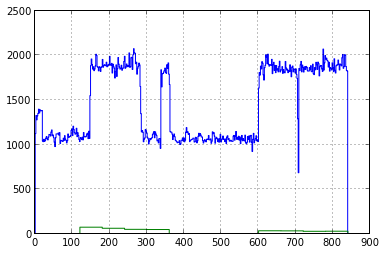
\includegraphics[width=0.7\textwidth]{parallel_files/parallel_fig_00.png}
\par
\end{center}
\end{codeoutput}
\end{codecell}
\begin{codecell}
\begin{codeinput}
\begin{lstlisting}
olap['s'] = olap['s'] - oltp['s'].min()
\end{lstlisting}
\end{codeinput}
\end{codecell}
\begin{codecell}
\begin{codeinput}
\begin{lstlisting}
olap[:10]
\end{lstlisting}
\end{codeinput}
\begin{codeoutput}
\begin{verbatim}
       tt          s         l
48106  12  60.782795  0.781321
48908  13  61.207099  0.424297
49365  18  61.910870  0.703767
50155  15  62.052910  0.142036
50318  21  63.025361  0.972447
51411  28  63.113924  0.088559
51500  14  63.440087  0.326159
51769  19  63.518115  0.078024
51824  15  63.656284  0.138165
51959  24  65.590104  1.933815
\end{verbatim}
\end{codeoutput}
\end{codecell}

\end{document}
